\setAuthor{Stanislav Zavjalov}
\setRound{lõppvoor}
\setYear{2012}
\setNumber{G 7}
\setDifficulty{8}
\setTopic{Termodünaamika}

\prob{Ahi}
\begin{wrapfigure}{r}{0.5\textwidth}%
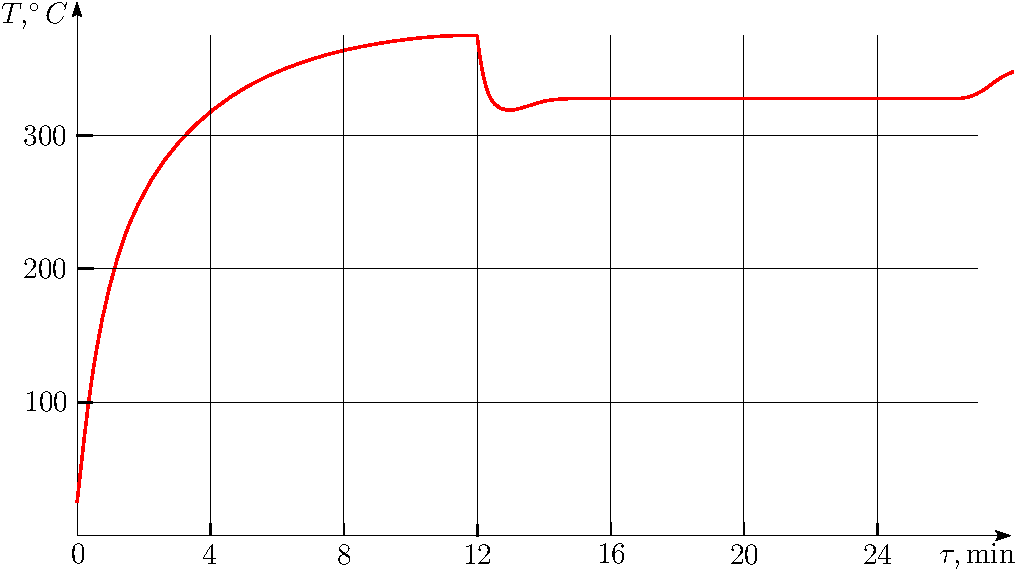
\includegraphics[width=\linewidth]{2012-v3g-07-ahi_graafik}%
\end{wrapfigure}
Väikese metallisulatusahju kütteelemendi võimsus on $P_0 = \SI{50}{W}$.
Toatemperatuuril olev ahi lülitakse sisse ja umbes 12 minuti pärast,
kui selle temperatuur praktiliselt enam ei kasva, pannakse ahju mitu
eelsoojendatud pliitükikest summaarse massiga $m = \SI{265}{g}$. Juuresoleval graafikul (suuremalt
lisalehel) on toodud
ahju temperatuuri sõltuvus ajast. Leidke selle põhjal plii sulamissoojus
$\lambda$.

\hint
On teada, et hetkeline efektiivne soojusvõimsus on võrdeline temperatuuri ja aja graafiku puutuja tõusuga. Enne pliitüki lisamist on ainsad soojuskaod läbi seinte; mida suurem on ahju temperatuur, seda suuremad on kaod. Pärast pliitüki lisamist läheb osa ahju võimsust veel plii sulatamiseks.

\solu
On teada, et hetkeline efektiivne soojusvõimsus on võrdeline temperatuuri ja aja graafiku puutuja tõusuga (ja võrdelisuskonstandiks on ahju soojusmahtuvus). Kuna esialgu on ahi toatemperatuuri juures, soojuskadusid esimestel hetketel peaaegu ei esine ja tiigli soojusvõimsusele $P_0 = \SI{50}{W}$ vastab puutuja tõus $\approx \SI{250}{\frac{^{\circ}C} {min}}$ (vt. joonist). On aga selge, et pika aja möödumisel tuleb soojuskadudega arvestada -- see ongi põhjus, miks ahju temperatuuri kasv kahaneb. Kui ahju sisse pannakse plii, langeb temperatuur kuni plii sulamistemperatuurini, $\approx \SI{327}{^\circ C}$ -- ahju kogu efektiivne võimsus kulub plii sulatamiseks (sest selle enda temperatuur ei muutu). Graafiku vasakult poolelt leiame, et temperatuuri $\approx \SI{327}{^\circ C}$ juures puutuja tõusuks oli $\approx \SI{45}{\frac{^{\circ}C} {min}}$, seega selle temperatuuri juures efektiivne võimsus on
\[
\frac{45}{250}P_0 \approx \num{0.18}P_0.
\]
Sellise võimsuse juures kuulub massi $m$ plii sulatamiseks $\Delta\tau \approx \SI{12}{min}$ aega (mille leiame graafikult). Seega, $\num{0.18} P_0 \Delta\tau = \lambda m$, kust
\[
\lambda = \frac{0,18 P_0 \Delta \tau}{ m} = \frac{0,18 \cdot \SI{50}{W} \cdot 12 \cdot \SI{60}{s}}{\SI{0.265}{kg}} = \SI{24.5}{\frac{kJ}{kg}}.
\]
\begin{center}
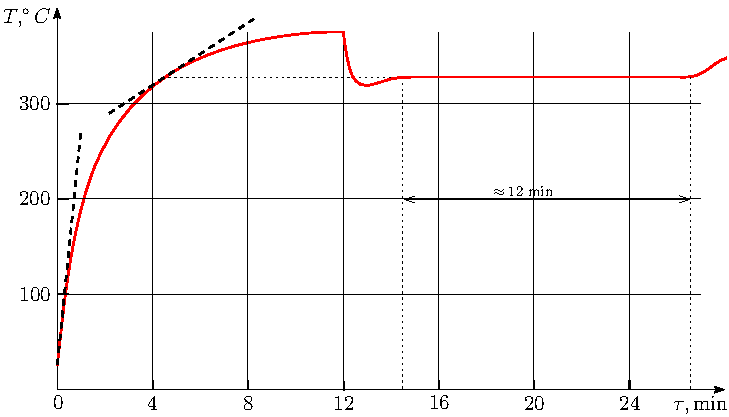
\includegraphics[width = 0.75\textwidth]{2012-v3g-07-ahi_lah}
\end{center}

\probeng{Furnace}
\begin{wrapfigure}{r}{0.5\textwidth}%
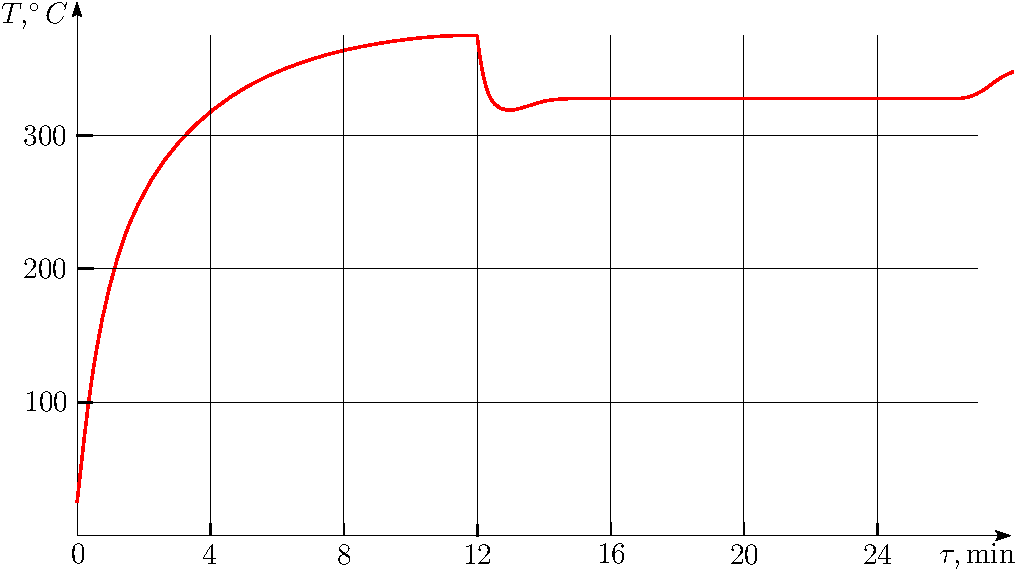
\includegraphics[width=\linewidth]{2012-v3g-07-ahi_graafik}%
\end{wrapfigure}
The power of a metal melting furnace’s heating element is $P_0 = \SI{50}{W}$. The furnace is turned on at room temperature and approximately after 12 minutes, when its temperature does not grow anymore, multiple preheated lead pieces with a total mass of $m = \SI{265}{g}$ are put into the oven. The relation between the temperature of the furnace and the time is shown in the figure. Based on that find the lead’s enthalpy of fusion $\lambda$.

\hinteng
It is known that instantaneous effective thermal power is proportional to the slope of the tangent of the temperature versus time graph. Before adding a lead piece the only heat losses are through the walls; the bigger the furnace’s temperature the bigger the losses. After adding a lead piece a part of the furnace’s power also goes to melting the lead.

\solueng
It is known that the momentary effective thermal power is proportional to the slope of the temperature and time graph’s tangent (and the proportionality constant is the furnace’s heat capacity). Because initially the furnace is at room temperature almost no heat losses occur in the first moments and the tangent slope $\approx \SI{250}{\frac{^{\circ}C} {min}}$ corresponds to the crucible’s thermal power $P_0 = \SI{50}{W}$  (see figure). It is, however, clear that after a long time has passed we need to take the heat losses into account – this is the reason why the furnace’s temperature growth decreases. If the lead is put inside the furnace the temperature falls to the lead’s melting temperature, $\approx \SI{327}{^\circ C}$ – the furnace’s total effective power goes to melting the lead (because its own temperature does not change). From the left side of the graph we find that at the temperature $\approx \SI{327}{^\circ C}$ the slope of the tangent was $\approx \SI{45}{\frac{^{\circ}C} {min}}$, therefore the effective power at this temperature is $\frac{45}{250}P_0 \approx \num{0.18}P_0$. At this power the time it takes to melt lead of mass $m$ is $\Delta\tau \approx \SI{12}{min}$ (which we find from the graph). Therefore, $\num{0.18} P_0 \Delta\tau = \lambda m$, where $\lambda = \frac{0,18 P_0 \Delta \tau}{ m} = \frac{0,18 \cdot \SI{50}{W} \cdot 12 \cdot \SI{60}{s}}{\SI{0.265}{kg}} = \SI{24.5}{\frac{kJ}{kg}}$.
\begin{center}
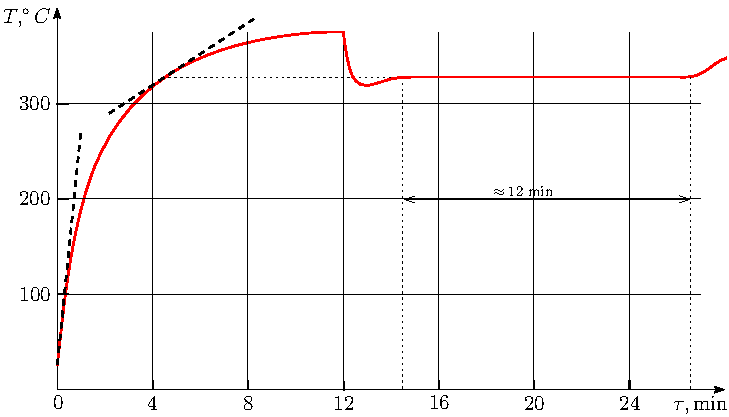
\includegraphics[width = 0.75\textwidth]{2012-v3g-07-ahi_lah}
\end{center}
\probend